\documentclass[12pt]{article}
\usepackage[margin=1in]{geometry}
\usepackage{amsmath, amssymb}
\usepackage{bm}
\usepackage{graphicx}
\usepackage{booktabs}
\usepackage{siunitx}
\usepackage{caption}
\usepackage{hyperref}
\usepackage{natbib}
% CJFR / Canadian Science Publishing author-date style: no comma between
% author and year in in-text citations, e.g. "(Paradis 2026)".
\setcitestyle{aysep={}}
\usepackage{titling}
\usepackage{longtable}
\usepackage{calc}
\providecommand{\tightlist}{\setlength{\itemsep}{0pt}\setlength{\parskip}{0pt}}

\pretitle{\begin{flushleft}\LARGE\bfseries}
\posttitle{\par\end{flushleft}\vskip 1em}
\preauthor{\begin{flushleft}\large}
\postauthor{\par\end{flushleft}\vskip 0.75em}
\predate{\begin{flushleft}\large}
\postdate{\par\end{flushleft}\vskip 1em}
\captionsetup[figure]{labelfont=bf,labelsep=space,name=Fig.}

\title{Dynamic inconsistency of promised future yields in open-loop LP forest plans: an open, reproducible benchmark of Daugherty (1991)}
\author{Gregory Paradis\\Department of Forest Resources Management, University of British Columbia, Canada\\Corresponding author: \texttt{gregory.paradis@ubc.ca}}
\date{\today}

\begin{document}

\maketitle

\noindent\textbf{Keywords:} non-declining yield; forest planning; linear programming; even flow; harvest scheduling; reproducibility; open-loop control; ws3

% !TEX root = ../main.tex
\begin{abstract}
Long-term timber harvest schedules produced by linear programming (LP) are routinely used in decision support. They are presented to decision-makers as credible statements about the future, and their shadow prices are used to value policy trade-offs. An open-loop LP solution is a plan made as if the planner could precommit to every future decision. However, real planning is sequential and adaptive: each period, the planner observes the realized forest state and re-solves. In a 1991 PhD thesis, P. J. Daugherty showed that LP forest plans solved open-loop admit \emph{dynamically inconsistent} plans. These plans fail Bellman's principle of optimality because a future planner re-solving from the realized state would not follow the plan's tail. We formalize dynamic inconsistency for LP forest plans with an operational divergence metric and provide the first open, reproducible benchmark of the phenomenon, reproducing and refining Daugherty's Umpqua National Forest FORPLAN case study in the open-source \texttt{ws3} model (Paradis 2026) from public planning documents. Across a grid of tested scenarios (18 landbases $\times$ 4 discount rates $\times$ 6 harvest-flow policies), dynamic inconsistency is pervasive under harvest-flow constraints (73\% of scenarios) yet largely absent without them at positive discount rates. The tested scenarios confirm that the formulation of the harvest volume flow constraint is the operative between-period link which drives the inconsistency. Inconsistency occurs at every discount rate, its magnitude is rate-dependent, and the non-declining-yield policy is the most inconsistent. On a landbase dominated by financially mature stands, the open-loop non-declining-yield plan promises a harvest flow that sequential replanning revises downward over most of the horizon, realizing today's harvests at the cost of future productive potentials. Four extension experiments test whether the phenomenon can be designed away: declining discount-rate schedules make it strictly more pervasive and introduce a preference-level (Strotz) inconsistency channel of their own; denominating the flow constraint in net revenue rather than volume doubles its magnitude while proving the negatively valued strata are a symptom rather than the cause; a rolling-mean flow floor shows that the replanning institution, not the constraint's shape, is the operative margin; and a max-harvest cap calibrated by iterative re-solve to a realized even-flow criterion eliminates the inconsistency entirely---at a credible harvest level measurably below the announced one. The presented model, data, and experiment are openly available and contribute to increased awareness of the risk of dynamically inconsistent LP solutions under even-flow constraints at the intersection of forest management planning, forest economics research, and decision support.
\end{abstract}

% !TEX root = ../main.tex
\section{Introduction}

Linear programming has been the workhorse of strategic forest planning for half a century. Since the Model~I and Model~II formulations of \citet{johnson1977techniques}, LP harvest-scheduling models, such as the USDA Forest Service's FORPLAN system and its successors, have been used to project long-term timber supply, to test harvest-flow policies, and to support trade-off analysis through the shadow prices that an optimal LP solution provides. In nearly all of such applications, the model is solved once, over the full multi-decade planning horizon, as an \emph{open-loop} problem: the entire sequence of future decisions is chosen at time zero, and the resulting schedule of harvest levels and residual forest structure is presented as the plan.

Real-world forest planning likely does not align with the open-loop assumption that today's planner could precommit to every future decision. Real planning is sequential: each period, the planner observes the realized forest state and re-solves the planning problem from that state, under the same objectives and constraints. If the tail of the original plan is not optimal for the subproblem that starts at the realized state, the re-solving planner will deviate from it. The announced plan then fails Bellman's principle of optimality \citep{bellman1957dynamic} and is \emph{dynamically inconsistent}. The projected harvest trajectory, residual growing stock, and shadow prices are not credible statements about what will or should happen. A plan that will not be followed cannot be a sound basis for long-term sustainable policies. Comparative analyses performed on it, including shadow-price trade-off analyses that often motivate such modelling studies, are biased.

This trap is a special case of a general phenomenon in dynamic economics: a plan that is optimal at time zero need not remain optimal at a later time, so a sequence of planners each re-optimizing from the realized state will not follow it \citep{strotz1956myopia,kydland1977rules}. It was demonstrated carefully and thoroughly for forest planning more than three decades ago. In his 1991 PhD thesis at the University of California, Berkeley, P. J. Daugherty proved analytically and demonstrated numerically that LP-based forest-planning models solved as open-loop formulations admit dynamically inconsistent plans, identified the structural conditions under which the inconsistency arises, and characterized its behaviour over a wide range of initial forest conditions and harvest policies \citep{daugherty1991credibility}. The thesis remains, to our knowledge, the most complete treatment of the problem in the forest-planning literature, yet it was never published in the peer-reviewed literature and is held only as an archival hard copy. The phenomenon itself has surfaced in the literature under various names, before and since---\citet{mcquillan1986declining} named the ``declining even-flow effect'' in national forest planning; \citet[pp.~331--332]{gunn2007models}, citing \citet{daugherty1991credibility}, calls it the ``declining non-declining yield''; and \citet{paradis2013risk} documented the systematic drift that arises between planned and implemented harvest under incoherent hierarchical planning, citing \citet{daugherty1991credibility} directly and using ``credibility'' in the thesis's sense. Yet the original analysis remains largely unread, and the field has lacked an open, citable, reproducible reference implementation against which to check it.

This paper formalizes dynamic inconsistency for LP forest plans and provides that reference. We present an open, transparent, and fully reproducible reproduction and refinement of the modelling methods and case study of \citet{daugherty1991credibility}, built on the open-source \texttt{ws3} wood-supply model \citep{paradis2026ws3} from the public-domain Umpqua planning documents (the 1987 Draft EIS and the 1990 FEIS Appendix B yield tables and economics). The contribution is fourfold. First, we give an operational divergence metric and occurrence criterion for dynamic inconsistency, making the phenomenon measurable and comparable across models. Second, we provide an open, test-backed \texttt{ws3} stack---the case-study data, the LP formulations, the sequential-replanning simulator, and the experiment grid---including a new \texttt{ws3} constraint form for the classic FORPLAN harvest-flow policies (non-declining yield and bounded sequential flow), released in \texttt{ws3} v1.1.0a5. Third, we reproduce and refine the thesis's empirical characterization across its full experiment grid (18 initial forest conditions $\times$ 4 discount rates $\times$ 6 harvest-flow policies), cleanly separating the harvest-flow constraint's role against a no-flow control and recovering the discount rate's occurrence-invariance and magnitude-dependence. Fourth---moving beyond reproduction---we run four pre-registered-style extension experiments, each asking the same question of a candidate modification: does it mitigate, or eliminate, the inconsistency? The variants probe the discount-rate \emph{shape} (declining-rate schedules), the flow constraint's \emph{denomination} (net revenue instead of volume) and \emph{shape} (rolling-mean rather than pointwise linkages, under two replanning institutions), and a \emph{cap-calibration} alternative that replaces the flow link with an iteratively tightened max-harvest cap. We emphasize the framing: the underlying science is a faithful reproduction of \citet{daugherty1991credibility}; the novelty is the operational metric, the open and reproducible benchmark, the rigorous driver diagnosis, and the systematic mitigation tests the open stack makes possible.

The remainder of this paper is organized as follows. Section 2 reviews the theory of dynamic inconsistency and the open-loop LP forest-planning problem, including the Model I/II/III formulation distinction. Section 3 describes the case study, the case-study data, the sequential-replanning simulator, the inconsistency metric, and the experiment design. Section 4 presents the reproduced results and the four extension experiments. Section 5 discusses the drivers of the inconsistency, the discount-rate nuance, implications for the literature, remedies, and limitations. Section 6 concludes.

% !TEX root = ../main.tex
\section{Background and theory}

\hypertarget{dynamic-inconsistency-and-bellmans-principle}{%
\subsection{Dynamic inconsistency and Bellman's principle}\label{dynamic-inconsistency-and-bellmans-principle}}

Consider a planner who at time zero chooses a sequence of decisions---here, harvest levels by stratum and period---over a finite horizon of \(T\) periods, so as to maximize an objective (discounted net present value, NPV) subject to constraints, including a harvest-flow constraint that links consecutive periods. The open-loop solution is a complete plan: a decision for every period, chosen once, at time zero, from the initial forest state.

Now suppose the plan is executed one period at a time by a sequence of planners, each inheriting the forest state realized by her predecessors and each solving the \emph{same} optimization problem from that state over the remaining horizon. Bellman's principle of optimality states that an optimal policy has the property that, whatever the initial state and initial decision, the remaining decisions must constitute an optimal policy with regard to the state resulting from the first decision \citep{bellman1957dynamic}. A plan that satisfies this property is \emph{dynamically consistent}: its tail is optimal for every subproblem it passes through, so each successive planner, re-solving from the realized state, voluntarily continues the plan. A plan that fails the property is \emph{dynamically inconsistent}: at some point the re-solving planner finds the plan's tail suboptimal for the state she has inherited and deviates from it. The open-loop projection of period-by-period harvests is then not a forecast of anything that will happen; it is a statement about a counterfactual world in which precommitment is possible.

Formally, let \(x = (x_1, \ldots, x_T)\) be a sequence of decisions and let the open-loop problem from state \(s_\tau\) over the remaining horizon be \(V_\tau(s_\tau) = \max_{x_\tau, \ldots, x_T} \sum_{t=\tau}^{T} \delta^{\,t-\tau} \, u_t(x_t)\) subject to the model's constraints, with \(\delta\) the per-period discount factor. The open-loop plan announced at time zero is \(x^{0} = (x_1^{0}, \ldots, x_T^{0}) = \arg\max V_1(s_1)\). Under sequential replanning, the planner at period \(\tau\) observes the realized state \(s_\tau = f(s_{\tau-1}, x_{\tau-1})\) (the forest left by her predecessor's decision) and re-solves \(V_\tau(s_\tau)\). The plan \(x^{0}\) is dynamically consistent if its tail is optimal for every subproblem it passes through, i.e., if \((x_\tau^{0}, \ldots, x_T^{0})\) remains a maximizer of \(V_\tau(s_\tau)\) for all \(\tau\); otherwise some planner deviates and the plan is not followed.

The practical stakes are not subtle. Long-term forest plans are used to set allowable cuts, to justify regulation of harvest flow, and to price constraints and land uses through shadow prices. If the plan is dynamically inconsistent, the projected harvest levels will not be delivered, the projected residual forest will not exist, and the shadow prices---which are properties of the particular optimal solution that will not be followed---are biased as measures of trade-offs along any trajectory that will actually occur.

\hypertarget{the-open-loop-lp-forest-planning-problem}{%
\subsection{The open-loop LP forest-planning problem}\label{the-open-loop-lp-forest-planning-problem}}

The standard strategic timber harvest-scheduling model is strata-based: the forest is partitioned into development types (strata) defined by attributes such as site, species composition, age, and management prescription, and the decision variables allocate stratum area to management activities over a horizon of discrete periods. The classical formulations are those of \citet{johnson1977techniques}. In \emph{Model I}, each existing stratum is assigned a complete management schedule as a distinct activity, so that the trajectory of every initial cohort is represented explicitly. In \emph{Model II}, decisions are expressed more compactly as area flows into a smaller set of prescription activities; \emph{Model III} aggregates further still, into a network flow over age classes. We refer the reader to \citep[ch.~16]{gunn2007models} for a careful statement of the Model I/II/III distinction and its lineage.

A word on model form and size is warranted, because a misconception about it circulates. Model II is widely described as the more compact formulation on the strength of its smaller variable count (Johnson and Scheurman 1977), and it is sometimes asserted that Model II reduces the size and difficulty of harvest-scheduling LPs relative to Model I. That expectation does not survive contact with modern instances. In the first published comparison of the two formulations on realistic spatial problems, \citet{martin2017comparing} showed that Model II's apparent compactness advantage evaporates---and reverses---once the problem carries realistic spatial resolution or many strata: Model II's per-strata constraint network makes its matrix denser and its solution time grow rapidly with added structure, while Model I's cost grows only marginally. On their full case study, Model I reached comparable optimal solutions in roughly a tenth of Model II's solution time. The authors' conclusion is blunt: the common expectation that Model II is the smaller, easier model is \emph{refuted} for all but the smallest or most weakly structured problems. This bears directly on the reproduction's formulation choice (below).

Two ingredients of the standard formulation matter for what follows. First, the objective is discounted NPV: timber values and costs in each period are weighted by a discount factor, so early harvest is preferred to late harvest, all else equal. Second, harvest-flow constraints---typically even-flow or bounded-deviation constraints on total volume between consecutive periods---create the only direct link between decisions in different periods. The economics of such harvest-flow constraints---the even-flow constraint and the allowable-cut effect it enables---have a long critical literature \citep{thompson1966traditional,schweitzer1972allowable,luckert1995allowable,hegan2000economic}. Without such a link, the multi-period problem decomposes and open-loop and sequential solutions coincide. With it, the current period's decision changes the feasible set---and the shadow prices---of every future subproblem.

Writing \(H_t\) for the total harvest volume in period \(t\) and suppressing the per-stratum detail, the open-loop problem maximizes discounted net revenue subject to a harvest-flow constraint linking consecutive periods:
\begin{equation}
\max_{H_1, \ldots, H_T \geq 0} \;\; \sum_{t=1}^{T} \delta^{\,t} \, r_t \, H_t
\qquad \text{s.t.} \qquad
(1 - \alpha)\, H_t \;\le\; H_{t+1} \;\le\; (1 + \beta)\, H_t, \;\; t = 1, \ldots, T-1,
\label{eq:openloop}
\end{equation}
where \(r_t\) is net revenue per unit volume in period \(t\) and \(\delta = (1+i)^{-1}\). The harvest-flow constraint is the classic FORPLAN bounded-deviation ("sequential flow") form \citep[eq.~3-4, 3-5]{daugherty1991credibility}: \(\alpha\) is the maximum allowed fractional \emph{decrease} and \(\beta\) the maximum allowed fractional \emph{increase} between consecutive periods. Its special cases span the standard harvest-flow policies: non-declining yield (\(\alpha = 0\), no increase bound; the yield may not fall), bounded decline (\(\alpha > 0\), no increase bound), and symmetric bounded deviation (\(\alpha = \beta > 0\)). It is this between-period link---and only this link---that prevents the multi-period problem from decomposing into independent single-period problems, and so it is the structural feature on which the consistency question turns.

\citet{daugherty1991credibility} conducted his analysis using a Model II formulation. The reproduction reported here builds the case study as a Model I model in \texttt{ws3}. The distinction matters for computational detail but not for the consistency question at issue: dynamic inconsistency is a property of the interaction among the objective, the flow constraint, and the initial forest structure, not of the variable-aggregation scheme. Moreover, the Model I choice is not merely a convenience: on the evidence of \citet{martin2017comparing}, Model I is at least as computationally efficient as Model II on realistic, well-structured problems, so nothing is sacrificed computationally by reproducing the analysis in the stand-based form. We nonetheless note the formulation difference explicitly as a fidelity caveat rather than a deviation of substance.

\hypertarget{daughertys-thesis}{%
\subsection{Daugherty's thesis}\label{daughertys-thesis}}

\citet{daugherty1991credibility} posed the credibility question directly: are the plans produced by LP-based forest-planning models, solved open-loop, plans that a sequence of future planners operating the same model would actually follow? The thesis (i) formalized dynamic consistency for LP forest-planning models, (ii) derived conditions under which open-loop optimal plans fail the consistency requirements, and (iii) demonstrated the phenomenon numerically by iterative LP simulation of sequential replanning on a real case study---the Umpqua National Forest FORPLAN planning model documented in \citep{usda1987umpqua}---across a designed experiment varying the initial forest condition, the harvest policy, and the interest rate. The thesis found dynamic inconsistency to be pervasive rather than exceptional, and traced it to the combination of the harvest-flow constraint with a disequilibrium initial forest containing financially over-mature and negatively valued strata. \citet[pp.~331--332]{gunn2007models}, citing \citet{daugherty1991credibility}, summarizes the practical symptom memorably as the ``declining non-declining yield'': a plan that promises a non-declining harvest trajectory while the sequential re-optimization it invites systematically revises the attainable harvest downward.

% !TEX root = ../main.tex
\section{Methods}

\hypertarget{case-study-the-umpqua-national-forest-forplan-model}{%
\subsection{Case study: the Umpqua National Forest FORPLAN model}\label{case-study-the-umpqua-national-forest-forplan-model}}

The case study reproduces the Umpqua National Forest FORPLAN planning model \citep{usda1987umpqua}, reconstructed in the open-source \texttt{ws3} wood-supply model \citep{paradis2026ws3}. The forest is stratified into four ecoclasses -- CH-CW, CD-CP, CR-CF, and CM-CE, dominated respectively by Douglas-fir, hemlock, fir, and hemlock types -- arrayed in decreasing growth potential. Seven silvicultural prescriptions are available, each with ecoclass-specific rotation-age ranges. The planning horizon is 150 years, divided into 15 periods of 10 years. The objective is maximization of net present value at a 4\% discount rate (varied in the experiments), with delivered-log prices escalating at 1\% per year for the first 50 years and constant thereafter. Volumes are expressed in thousands of cubic feet (MCF). The harvest-flow policy is the thesis's bounded-deviation \emph{sequential-flow} constraint of equation~\eqref{eq:openloop}, tying each period's total harvest volume to the previous period's; the specific policy levels are the thesis's six harvest-flow constraint sets (Section~\ref{experiment-design}). The initial forest is specified as one of a set of landbase conditions; the landbase of central interest (landbase 1) is an all-mature forest, the extreme of the disequilibrium structures the thesis studies.

\hypertarget{case-study-data}{%
\subsection{Case-study data}\label{case-study-data}}

The case study is built from the real Umpqua FORPLAN data, obtained from the public-domain Umpqua National Forest planning documents on HathiTrust. The per-age yield curves -- the volume removed per acre by age for each ecoclass, prescription, and management intensity -- come from the 1990 Final Environmental Impact Statement (FEIS) Appendix B \citep{usda1990umpqua} (the FORPLAN analysis volume: managed yield tables generated with the DFSIM Douglas-fir simulator, with operational-falldown adjustments, and the mountain-hemlock curve from Johnson's mountain-hemlock site equations). The economics come from the FEIS's timber-value derivations: stumpage, logging, and manufacturing costs by species (its Table B-65), the Douglas-fir price-diameter and pond-value relationships (Table B-66), and the per-ecoclass access (road) costs that make the high-elevation mountain-hemlock (CM-CE) prescriptions negatively valued. The yield-curve shapes are consistent with the LRMP's documented 95\% CMAI culmination ages by ecoclass (its Table IV-3: 85 years for CH-CW, 120 for CD-CP, 115 for CR-CF, 175 for CM-CE), and the FEIS Stage II financial analysis corroborates the thesis's anchor values (its mature-timber NPV range of \$1,800--\$7,700 per acre brackets the thesis's Table 5.4 mature-type NPVs; its managed-prescription range of \$27--\$290 per acre and the negative mountain-hemlock values match the thesis's Table 5.3 ordering and signs).

All source documents were obtained and machine-read from HathiTrust (public domain): the 1990 LRMP, the 1990 FEIS main volume and its Appendix B (the FORPLAN analysis volume), and the 1987 Draft EIS \citep{usda1987umpqua} that Daugherty used directly (the thesis's exact data vintage). The 1987 DEIS and 1990 FEIS yield tables agree, so the assembled case study uses Daugherty's exact data. The case study reproduces the thesis's printed anchor tables (Tables 5.3 and 5.4): the five mature vegetation types' model PNVs match their Table 5.4 anchors exactly (their standing volumes are set so that volume $\times$ the FEIS net delivered-log price equals the anchor), and the managed prescriptions match Table 5.3 in sign and broad rotation range (the exact optimal-rotation ordering is only partially reproduced, as the FEIS prescription mapping simplifies some treatments; Section 5.5). Because the mature volumes are derived from the Table 5.4 anchors, we additionally cross-check them against an independent source -- the FEIS standing-volume-by-age curves at each mature type's age -- which agree in order of magnitude. All data are typed, provenance-stamped records in the repository; the extraction of the FEIS Appendix B tables is a one-time, documented, reproducible step, and the package does not depend on the scanned source at runtime.

\hypertarget{the-sequential-replanning-simulator}{%
\subsection{The sequential-replanning simulator}\label{the-sequential-replanning-simulator}}

Dynamic inconsistency cannot be observed in a single open-loop solve; it is defined by what happens when the plan meets sequential re-optimization. Following the thesis's iterative LP simulation, we implement a sequential-replanning simulator:

\begin{enumerate}
\def\labelenumi{\arabic{enumi}.}
\tightlist
\item
  Solve the open-loop LP from the current forest state over the horizon.
\item
  Apply the current period's decision from that solution.
\item
  Advance the forest state by one period: the realized area-by-age distribution is extracted from the model and becomes the initial condition of the next subproblem.
\item
  Re-solve the open-loop LP from the realized state over the (rolling) horizon.
\item
  Repeat to the end of the simulation, recording both the plan projected at each step and the decisions actually taken.
\end{enumerate}

Two modeling decisions bear on the interpretation and are worth stating explicitly. First, each replan re-solves the harvest-scheduling problem with a \emph{fresh} harvest-flow constraint anchored to that subproblem's own trajectory, not carried from the prior period's realized harvest. This is the faithful reading of FORPLAN practice -- each decadal re-solve is a new plan with its own flow constraint -- and it is what allows the promised non-declining flow to be abandoned (the phenomenon). The alternative convention (anchoring each replan's first period to the realized previous harvest, i.e., carrying the flow-history as a standing rule) suppresses the phenomenon by forcing the realized trajectory to track the plan until the constraint becomes infeasible; we implemented it as an option and report the rolling- versus shrinking-horizon and reset conventions as a robustness consideration. Second, because LP optima can be non-unique, a divergence between the projected and realized harvest vectors could in principle reflect an alternate optimum rather than genuine inconsistency. To rule this out we add an \emph{objective-gap diagnostic}: at each replan we solve the subproblem freely and again with the period-1 harvest held to the announced plan's value (within a 1\% band), and we compare the two objectives. If the re-solved objective strictly exceeds the tail-fixed objective -- or the announced value is infeasible from the realized state -- the announced plan's tail is strictly suboptimal or unimplementable, i.e., genuinely dynamically inconsistent, not merely a different member of an optimal set.

The inconsistency measure is the divergence between the open-loop plan's projected per-period harvest and the realized replanned trajectory -- that is, the changes in decisions and in projected output levels over time between what was announced and what the re-solving planner actually does. Formally, with the open-loop projection \(p = (p_1, \ldots, p_T)\) and the realized replanned trajectory \(r = (r_1, \ldots, r_T)\), we measure the per-period divergence by the symmetric relative deviation
\begin{equation}
\delta_t = \frac{|p_t - r_t|}{\max(|p_t|, |r_t|, \varepsilon)},
\label{eq:metric}
\end{equation}
which is bounded in \([0, 1]\) and robust to near-zero harvest baselines, and summarize a cell by its mean \(\bar\delta = \frac{1}{T}\sum_t \delta_t\) and by the relative change in total volume \((\sum_t r_t - \sum_t p_t)/\sum_t p_t\). A cell exhibits dynamic inconsistency when \(\bar\delta\) exceeds a small tolerance (5\%, well above LP-solver numerical noise and well below the observed magnitudes). The first-period decision is consistent by construction (the realized period-1 harvest is the open-loop period-1 decision), so the divergence is in the plan's tail, as the theory predicts. The simulator supports a rolling fixed horizon (the default, which avoids the terminal artifacts of a shrinking horizon) and a shrinking-horizon variant; all seed-dependent runs are fixed-seeded and bit-stable.

\hypertarget{experiment-design}{%
\subsection{Experiment design}\label{experiment-design}}

The experiment grid reproduces the thesis's three experimental factors: initial forest condition (landbase), harvest policy, and the interest rate. The reproduced grid spans \emph{all eighteen} of the thesis's initial forest conditions \citep[Table~5.5]{daugherty1991credibility}: the all-mature landbases (1, and 2 excluding the negatively valued CM-CE ecoclass); the area-control-derived landbases (3--8: landbase 1 or 2 after 40 or 70 years of area-control harvest at a 70- or 100-year rotation, a disequilibrium\(\to\)regulation gradient); the structured young-growth landbases (9, equal acres by age class; 10, unequal); and the randomly generated young-growth landbases (11--18, seed-fixed). Harvest policy is the thesis's six harvest-flow constraint sets \citep[Table~5.6]{daugherty1991credibility}: no harvest flow (NHF, the control); non-declining yield (NDY); bounded decline of 10\% or 20\% (\(-10\%\), \(-20\%\)); and symmetric bounded deviation of 10\% or 20\% (\(\pm10\%\), \(\pm20\%\)). The discount rate takes the thesis's four values (0\%, 2\%, 4\%, 6\%). Each of the 432 cells is a full sequential-replanning simulation under the cell's policy (equation~\eqref{eq:openloop}), scored for the occurrence and magnitude of dynamic inconsistency (equation~\eqref{eq:metric}). The grid is run by a tracked entry point and is embarrassingly parallel. (The thesis re-solved for eleven periods over its planning horizon; we run the full fifteen-period horizon, a refinement that extends the observation window without changing the mechanism.)

The thesis also used ending-period (terminal) constraints -- ending inventory at least 80\% of the regulated forest's average inventory, and final-period harvest at most 120\% of long-term sustained yield -- with its flow-constrained runs, to minimize horizon effects. We implemented and tested these; with the corrected case-study data the model does not exhibit the horizon-end liquidation they guard against, so they are non-binding here and are omitted from the reported grid (they remain available and are flagged experimental in the stack).

\hypertarget{implementation-and-reproducibility}{%
\subsection{Implementation and reproducibility}\label{implementation-and-reproducibility}}

The complete stack -- typed, provenance-recorded case-study data; the \texttt{ws3} forest model; the explicit LP builder; the sequential-replanning simulator; the experiment runner; and the validation records -- is openly available (see Software availability). The thesis's bounded-deviation sequential-flow harvest-flow constraint (equation~\eqref{eq:openloop}) required a new even-flow constraint form in \texttt{ws3} (consecutive-period anchoring with separate decrease/increase tolerances), contributed upstream and released in \texttt{ws3} v1.1.0a5; it is a reusable addition for the classic FORPLAN harvest-flow policies. The package is test-backed, the environment is locked, and the simulation records needed to regenerate every number reported below are produced by the repository's experiment entry points.

% !TEX root = ../main.tex
\section{Results}

We report the reproduced findings of the full experiment grid (18 landbases $\times$ 4 discount rates $\times$ 6 harvest-flow policies; 432 sequential-replanning simulations). Per the framing of this paper, these reproduce and refine \citet{daugherty1991credibility}'s findings on the real Umpqua FORPLAN case study; they are presented with their fidelity caveats in Section 5. Every number below is regenerated by the repository's tracked experiment entry point; the per-cell simulation records are the tracked benchmark record (\texttt{results/experiments/}), summarized with figures and tables in the curated supplement (\texttt{supplementary/02-core-grid.md}).

\textbf{The harvest-flow constraint is the operative link.} Dynamic inconsistency is pervasive under the harvest-flow policies but largely absent without one. Across the grid, 73\% of the flow-constrained cells (NDY, bounded decline, and bounded deviation) exhibit inconsistency by the divergence metric (equation~\eqref{eq:metric}), against 38\% of the no-harvest-flow (NHF) control cells -- and the NHF divergence is concentrated at the lowest discount rates (0--2\%), where the objective is nearly indifferent to timing; at 4--6\% the no-flow control is consistent (Section 5). In all flow-constrained cells the first-period decision is consistent -- the divergence is in the plan's tail, exactly as the theory predicts. Where a model links periods only through a harvest-flow constraint, its projected harvest trajectory is a property of a plan that sequential re-optimization will not follow.

\textbf{The declining non-declining yield.} On the all-mature landbase 1, the divergence between announcement and delivery is stark (Figure~\ref{fig:ndy}). The open-loop non-declining-yield plan projects a smooth, credible-looking level harvest flow; the realized replanned trajectory is revised downward over most of the horizon as each successive planner inherits the depleted forest and re-solves. This is the ``declining non-declining yield'' of \citet[pp.~331--332]{gunn2007models}: the promised non-declining flow declines precisely because each successive planner declines to honour it.

\begin{figure}[t]
\centering
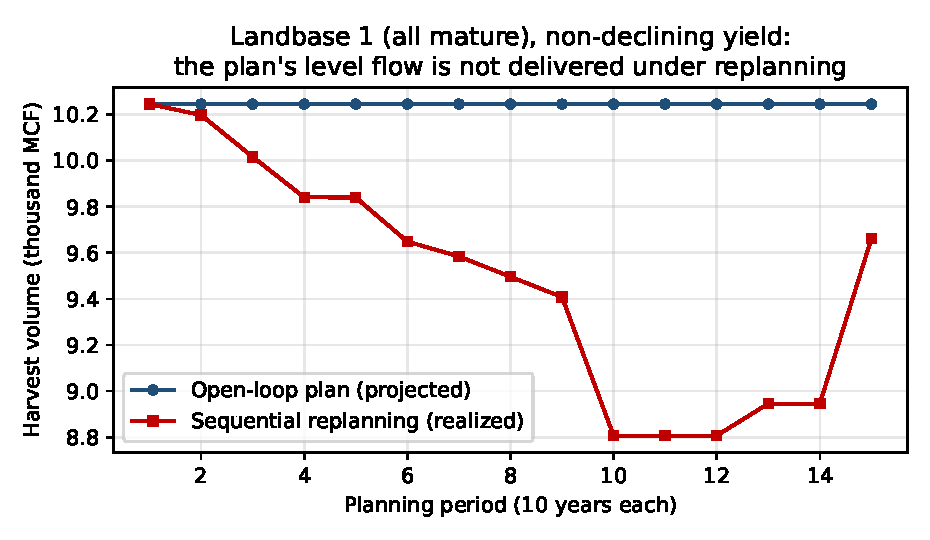
\includegraphics[width=\textwidth]{figures/fig_declining_ndy.pdf}
\caption{The declining non-declining yield on the all-mature landbase 1 under the non-declining-yield (NDY) harvest-flow policy at a 4\% discount rate. The open-loop plan projects a level, non-declining harvest flow; the realized sequential-replanning trajectory is revised downward over most of the horizon. Full provenance and the per-cell simulation records: \texttt{results/experiments/grid\_trajectories.csv}; supplement \texttt{supplementary/02-core-grid.md}.}
\label{fig:ndy}
\end{figure}

\textbf{Occurrence at every discount rate; magnitude is rate-dependent.} Inconsistency occurs at every discount rate in the grid (the flow-constrained occurrence rate is 100\% at 0\% and 47--86\% at 2--6\%), consistent with the thesis's analytical result that, because the discount factor is uniform across periods, it drops out of the consistency requirements \citep[ch.~3, p.~58--59]{daugherty1991credibility} -- the phenomenon does not require a particular rate. The \emph{magnitude} is rate-dependent: on landbase 1 under NDY, the mean relative divergence and the total-volume shortfall are markedly larger at a 0\% rate (where the objective is indifferent to timing) than at 2--6\%. We return to this nuance in the Discussion, because it refines -- rather than contradicts -- the naive account of the phenomenon.

\textbf{The divergence is genuine inconsistency, not an artifact of alternate optima.} Because LP optima can be non-unique, a divergence between the projected and realized trajectories could in principle reflect a different member of an optimal set rather than a plan that will not be followed. The objective-gap diagnostic (Section 3.3) rules this out: it re-solves each subproblem freely and again with the period-1 harvest held to the announced plan's value, and compares the objectives. On landbase 1 under NDY, the announced plan's tail is strictly suboptimal or outright infeasible from the realized state in 13--14 of 15 replan periods at every discount rate -- the re-solving planner strictly improves on, or cannot even implement, the announced tail. Under the no-flow control, by contrast, the announced tail remains optimal at every period at 4--6\% (and largely optimal at 0\%, where the flat objective admits alternate optima). The inconsistency is therefore a property of the flow-constrained plan, not of solver tie-breaking.

\textbf{Effect of the harvest-flow policy.} The strictness and form of the flow constraint shape the inconsistency. The non-declining-yield policy -- permitting no decrease -- produces the most frequent divergence (occurrence 86\%, the highest of the flow policies), and the magnitude of the divergence varies by policy and landbase (Table 1). At the base and higher discount rates (4--6\%) the no-flow control is consistent (0\% occurrence), confirming the flow constraint as the operative between-period link; at the lowest rates (0--2\%) the no-flow control also diverges, which we attribute to timing-indifference (a near-flat objective admits near-tie optima that the re-solver resolves differently) rather than genuine inconsistency -- the objective-gap diagnostic (Section 3.3) confirms the no-flow tail remains optimal there.

\textbf{Role of disequilibrium structure.} The inconsistency occurs across all eighteen initial forest conditions (flow-constrained occurrence 50--100\% by landbase), and is most pronounced in magnitude on the disequilibrium structures: the all-mature and area-control-derived landbases, which place a pulse of immediately harvestable, financially over-mature volume in front of a regulated future that cannot sustain it. The CM-CE ecoclass is negatively valued -- its harvest cost exceeds its timber value -- and such strata enter the open-loop solutions as \emph{inconsistent variables}: area allocations whose only function is to relax the binding flow constraint in the plan and that the re-solving planner subsequently abandons.

\textbf{Table 1.} Experiment-grid summary: factors, levels, occurrence of dynamic inconsistency (share of cells exceeding the 5\% divergence tolerance), and mean magnitude (symmetric relative deviation, equation~\eqref{eq:metric}), over the full grid (432 cells). Full per-cell simulation records: \texttt{results/experiments/grid.csv}; per-landbase detail in \texttt{supplementary/04-landbases.md}.

\begin{table}[h]
\centering
\small
\begin{tabular}{@{}llcc@{}}
\toprule
Factor & Levels & Occurrence & Mean magnitude \\
\midrule
Harvest-flow policy & NDY, $-10\%$, $-20\%$, $\pm10\%$, $\pm20\%$ & 58--86\% & 0.10--0.13 \\
\quad (control) & NHF (no harvest flow) & 38\% & 0.13 \\
Discount rate & 0\%, 2\%, 4\%, 6\% & 100\% / 47--86\% & rate-dependent \\
Initial forest condition & 18 landbases (Table 5.5) & 50--100\% & 0.08--0.23 \\
\bottomrule
\end{tabular}
\end{table}

% !TEX root = ../main.tex
\section{Discussion}

\hypertarget{what-drives-the-inconsistency}{%
\subsection{What drives the inconsistency}\label{what-drives-the-inconsistency}}

The reproduction cleanly separates the ingredients of the phenomenon. The harvest-flow constraint is the operative between-period link: without it, the announced plan's tail remains optimal at each replan (the objective-gap diagnostic confirms the no-flow control is consistent at positive discount rates), and with it the re-solving planner strictly improves on -- or cannot even implement -- the announced tail. The non-declining-yield policy, the most restrictive, is the most frequently inconsistent. The disequilibrium forest structure is the fuel: a mature/old-growth landbase places a large pulse of immediately harvestable, financially over-mature volume in front of a regulated future that cannot sustain it, so the open-loop plan's promised smooth flow can only be constructed by commitments the future planner will not keep. The negatively valued strata are the tell: because CM-CE area enters the solution only to mitigate the binding flow constraint and is then abandoned under replanning, its presence in the open-loop solution is a direct, observable marker of the inconsistency rather than a real management intention.

\hypertarget{the-discount-rate-nuance}{%
\subsection{The discount-rate nuance}\label{the-discount-rate-nuance}}

One finding deserves emphasis because it is easy to misstate. The naive account -- ``a discounted objective plus an even-flow constraint breaks Bellman's principle'' -- suggests that the discount rate is the operative driver and that consistency could be restored by lowering it. The reproduction shows this is not so: genuine dynamic inconsistency -- the announced plan's tail being strictly suboptimal or infeasible from the realized state, per the objective-gap diagnostic (Section 3.3) -- occurs at every discount rate (0\%, 2\%, 4\%, and 6\%) for the flow-constrained policies. The resolution is in the thesis itself \citep[ch.~3, p.~58--59]{daugherty1991credibility}: because the discount factor is uniform across periods, it cancels out of the conditions that a plan must satisfy to be consistent, so the \emph{occurrence} of inconsistency does not require a particular rate. Discounting shapes \emph{which} plan is chosen and the \emph{magnitude} of the divergence, however: the mean relative divergence and total-volume shortfall are markedly larger at a 0\% rate than at 2--6\%. We note one subtlety the metric alone would obscure: at a 0\% rate the flat objective admits near-tie optima, so the trajectory-divergence metric also flags the no-flow control (whose announced tail the objective-gap diagnostic shows is largely still optimal there -- alternate optima, not genuine inconsistency); at positive rates the objective discriminates and the flow-constraint divergence is genuine. So the rate matters to the plan and to how badly the plan is wrong, but not to whether the plan is wrong. We present this as a reproduced nuance of the thesis, not as a contradiction of it -- recovering this counter-intuitive rate-independence on independent software is a meaningful check that the reproduction has captured the thesis's mechanism. The practical corollary is uncomfortable: discount-rate policy is not a remedy for non-credible plans.

\hypertarget{implications-for-the-literature}{%
\subsection{Implications for the literature}\label{implications-for-the-literature}}

The implication for the large literature of open-loop LP forest-planning studies -- and for planning practice built on single-solve strategic models -- is direct. Where a model combines a harvest-flow constraint with a disequilibrium initial forest, its projected harvest trajectories, residual growing-stock trajectories, and shadow prices are properties of a plan that sequential re-optimization will not follow, and trade-off analysis conducted on them is biased. The ``declining non-declining yield'' \citep[pp.~331--332]{gunn2007models} names the symptom exactly: the promised non-declining flow declines precisely because each successive planner declines to honour it. The same mechanism surfaces downstream, in the hierarchical link between strategic and operational planning: \citet{paradis2013risk} showed that incoherent linkage between long-term wood-supply allocation and short-term harvest planning induces a systematic drift between planned and implemented harvest (a divergence of forest system state), citing \citet{daugherty1991credibility} and naming the declining-non-declining-yield phenomenon. The dynamic inconsistency reproduced here is the analytic root of that practical drift, a connection to the longer economics literature on the even-flow constraint and the allowable-cut effect \citep{thompson1966traditional,schweitzer1972allowable,luckert1995allowable,hegan2000economic}. That the underlying analysis was never peer-reviewed and has been held only as an archival thesis plausibly explains why the phenomenon has been repeatedly rediscovered; an open, citable, reproducible reference implementation is useful to the field.

\hypertarget{remedies}{%
\subsection{Remedies}\label{remedies}}

The thesis and the subsequent literature point to three families of remedies, which the reproduction makes concrete. First, \emph{consistent formulations}: rather than solving one open-loop problem, compute solutions that are optimal for the sequential game the planning process actually is -- subgame-perfect or feedback solutions in which each period's decision is optimal given the state and the continuation policy. The thesis discusses the generation of consistent solutions; computing them exactly for the full case study is a natural follow-on enabled by this stack. Second, \emph{credible precommitment}: inconsistency arises because the future planner is free to re-solve; institutional commitments that genuinely bind future decisions -- for example, regeneration mandates attached to harvest -- change the future subproblem and can restore credibility to announced plans; the principal-agent literature on incentive-compatible timber-supply policy after disturbance develops this incentive-compatibility angle \citep{bogle2015protecting}. Third, \emph{receding-horizon practice with honest reporting}: if planning is in fact sequential replanning, then the simulator used here -- not the single open-loop solve -- is the honest model of what the planning process will deliver, and plan documents should report the realized replanned trajectory rather than the open-loop projection.

\hypertarget{limitations}{%
\subsection{Limitations}\label{limitations}}

Several limitations bound the claims. First, the data vintage: the case study is built from the 1990 FEIS (the FORPLAN model lineage with updated 1980s prices), cross-checked against the 1987 DEIS that Daugherty used directly; the two vintages' yield tables agree, and the thesis's exact base-case schedule is not matched period by period because the thesis's per-period realized schedule is not printed. Validation is against the thesis's printed anchors: the mature-type PNVs match Table 5.4 exactly (their volumes are derived from the anchors, cross-checked against the independent FEIS standing-volume curves), and the managed prescriptions match Table 5.3 in \emph{sign} and broad rotation range (the exact optimal-rotation ordering is only partially reproduced -- the FEIS prescription mapping simplifies some treatments). Second, the formulation caveat: the thesis used a Model II formulation; the reproduction uses Model I (Section 2.2), because the Model II flow-constraint compilation is not yet implemented in \texttt{ws3} -- a forced substitution whose behavioral equivalence under sequential replanning we note but do not demonstrate. Third, the thesis used ending-period (terminal) constraints with its flow-constrained runs to minimize horizon effects; we implemented these in the stack (currently opt-in and experimental) and found that with the corrected case-study data the model does not exhibit the horizon-end liquidation they guard against, so they are omitted from the reported grid. Fourth, the simulator is a rolling-horizon (receding-horizon) institution, which is how planning actually proceeds; a shrinking-horizon variant (the pure Bellman tail over a fixed terminal date) shows the same qualitative phenomenon at somewhat smaller magnitude (on landbase 1 under NDY at 4\%, mean relative divergence 0.050 shrinking vs 0.074 rolling; both inconsistent). Fifth, scope: this is one case study. The pervasiveness result (73\% of flow-constrained cells) is a property of this grid, and extension to other forests, formulations, and consistent-solution constructs is future work -- work that the open stack is intended to make easy.

% !TEX root = ../main.tex
\section{Conclusion}

The core result of \citet{daugherty1991credibility} holds, and it is now formalized, reproducible, and citable. LP forest-planning models solved as open-loop formulations with a harvest-flow constraint, applied to disequilibrium forest structures containing negatively valued strata, produce dynamically inconsistent plans: a future planner re-solving from the realized state under the same objectives will not follow the plan's tail. Across the thesis's full experiment grid, the inconsistency is pervasive under the harvest-flow policies (73\% of cells) yet largely absent without one at positive discount rates -- the no-flow control is consistent at 4--6\% -- confirming the harvest-flow constraint as the operative between-period link; and, reproducing the thesis's subtlest finding, inconsistency occurs at every discount rate while its magnitude is rate-dependent. On the all-mature landbase, the open-loop non-declining-yield plan's smooth, credible-looking level flow gives way under sequential replanning to a realized trajectory that is revised downward over most of the horizon. A plan that will not be followed is not a credible basis for policy, and shadow-price analysis computed from it is biased. The contribution of this paper is an operational divergence metric, an open and fully reproducible quantitative benchmark of the phenomenon on the thesis's complete experiment grid, a rigorous driver diagnosis, and a reusable \texttt{ws3} stack -- including a new sequential-flow even-flow constraint form -- that make a three-decades-old, never-peer-reviewed result available for verification, citation, teaching, and extension, including the consistent-formulation and precommitment remedies that the thesis pointed toward and that the stack now makes computable in public.

% !TEX root = ../main.tex
\section{Software availability}

All software, extracted case-study data, experiment configurations, simulation records, and the validation records supporting this paper are openly available in the \texttt{fresh-daugherty} repository \citep{freshdaugherty}. The stack is built on the open-source \texttt{ws3} wood-supply model \citep{paradis2026ws3}. A companion reproduction of a related dynamic-inconsistency test instance is maintained in the \texttt{fresh-fuchs} repository \citep{freshfuchs}.


\section*{Acknowledgements}
Development of this work was supported by the Forest Resources Environmental Services Hub (FRESH) at the University of British Columbia. LLM-assisted tools contributed to code development and editing; the author reviewed and approved all content.

\section*{Author contributions}
G. Paradis designed the study, performed the analysis, and prepared the manuscript.

\section*{Competing interests}
The author is the developer of the open-source \texttt{ws3} framework used and extended in this work, and the paper provides a citable reference for it -- a non-financial competing interest declared in the interest of transparency. The author declares no financial competing interests.

\section*{Data availability}
All software, extracted case-study data, experiment configurations, the full per-cell simulation records, and the validation records supporting this paper are openly available in the \texttt{fresh-daugherty} repository at \url{https://github.com/UBC-FRESH/fresh-daugherty}. The complete benchmark record -- the grid summary and the per-cell projected and realized harvest trajectories for all 432 cells, together with the exact regeneration command and pinned dependency versions -- is tracked under \texttt{results/experiments/} and archived with a DOI at \url{https://doi.org/10.5281/zenodo.21981434} (release v0.1.0b1). The Umpqua planning documents are public-domain US Forest Service works accessible via HathiTrust (records 002547999 and 002439528).

\bibliographystyle{apalike-doi}
\bibliography{references}

\end{document}
